\documentclass[11pt]{beamer}\usepackage[]{graphicx}\usepackage[]{color}
%% maxwidth is the original width if it is less than linewidth
%% otherwise use linewidth (to make sure the graphics do not exceed the margin)
\makeatletter
\def\maxwidth{ %
  \ifdim\Gin@nat@width>\linewidth
    \linewidth
  \else
    \Gin@nat@width
  \fi
}
\makeatother

\definecolor{fgcolor}{rgb}{0.345, 0.345, 0.345}
\newcommand{\hlnum}[1]{\textcolor[rgb]{0.686,0.059,0.569}{#1}}%
\newcommand{\hlstr}[1]{\textcolor[rgb]{0.192,0.494,0.8}{#1}}%
\newcommand{\hlcom}[1]{\textcolor[rgb]{0.678,0.584,0.686}{\textit{#1}}}%
\newcommand{\hlopt}[1]{\textcolor[rgb]{0,0,0}{#1}}%
\newcommand{\hlstd}[1]{\textcolor[rgb]{0.345,0.345,0.345}{#1}}%
\newcommand{\hlkwa}[1]{\textcolor[rgb]{0.161,0.373,0.58}{\textbf{#1}}}%
\newcommand{\hlkwb}[1]{\textcolor[rgb]{0.69,0.353,0.396}{#1}}%
\newcommand{\hlkwc}[1]{\textcolor[rgb]{0.333,0.667,0.333}{#1}}%
\newcommand{\hlkwd}[1]{\textcolor[rgb]{0.737,0.353,0.396}{\textbf{#1}}}%

\usepackage{framed}
\makeatletter
\newenvironment{kframe}{%
 \def\at@end@of@kframe{}%
 \ifinner\ifhmode%
  \def\at@end@of@kframe{\end{minipage}}%
  \begin{minipage}{\columnwidth}%
 \fi\fi%
 \def\FrameCommand##1{\hskip\@totalleftmargin \hskip-\fboxsep
 \colorbox{shadecolor}{##1}\hskip-\fboxsep
     % There is no \\@totalrightmargin, so:
     \hskip-\linewidth \hskip-\@totalleftmargin \hskip\columnwidth}%
 \MakeFramed {\advance\hsize-\width
   \@totalleftmargin\z@ \linewidth\hsize
   \@setminipage}}%
 {\par\unskip\endMakeFramed%
 \at@end@of@kframe}
\makeatother

\definecolor{shadecolor}{rgb}{.97, .97, .97}
\definecolor{messagecolor}{rgb}{0, 0, 0}
\definecolor{warningcolor}{rgb}{1, 0, 1}
\definecolor{errorcolor}{rgb}{1, 0, 0}
\newenvironment{knitrout}{}{} % an empty environment to be redefined in TeX

\usepackage{alltt}

\makeatletter
\def\maxwidth{ %
  \ifdim\Gin@nat@width>\linewidth
    \linewidth
  \else
    \Gin@nat@width
  \fi
}
\makeatother

\definecolor{shadecolor}{rgb}{.97, .97, .97}
\definecolor{messagecolor}{rgb}{0, 0, 0}
\definecolor{warningcolor}{rgb}{1, 0, 1}
\definecolor{errorcolor}{rgb}{1, 0, 0}

\usepackage{alltt}
\usepackage{natbib}
\usepackage{array}
\usepackage[font=small,skip=5pt]{caption}
\usepackage{graphicx}
\usepackage{amsmath}
\usepackage{dsfont}
\usepackage[]{algorithm2e}
\usepackage{amsthm}
\usepackage{amsfonts}
\usepackage{url}
\usepackage{ulem}
\usepackage{afterpage}
\usepackage{bbm}
\usepackage{tikz}
\usepackage{amssymb}
\usepackage{bm}
\setbeamertemplate{caption}[numbered]

\usetheme{Warsaw}
\defbeamertemplate*{footline}{shadow theme}
{%
  \leavevmode%
  \hbox{\begin{beamercolorbox}[wd=.5\paperwidth,ht=2.5ex,dp=1.125ex,leftskip=.3cm plus1fil,rightskip=.3cm]{author in head/foot}%
    \usebeamerfont{author in head/foot}\insertframenumber\,/\,\inserttotalframenumber\hfill\insertshortauthor
  \end{beamercolorbox}%
  \begin{beamercolorbox}[wd=.5\paperwidth,ht=2.5ex,dp=1.125ex,leftskip=.3cm,rightskip=.3cm plus1fil]{title in head/foot}%
    \usebeamerfont{title in head/foot}\insertshorttitle%
  \end{beamercolorbox}}%
  \vskip0pt%
}

\setbeamertemplate{headline}{%
\leavevmode%
  \hbox{%
    \begin{beamercolorbox}[wd=\paperwidth,ht=2.5ex,dp=1.125ex]{palette quaternary}%
    \insertsectionnavigationhorizontal{\paperwidth}{\hskip0pt plus1filll}{\hskip0pt plus1filll}
    \end{beamercolorbox}%
  }
}

\newcounter{saveenumi}
\newcommand{\seti}{\setcounter{saveenumi}{\value{enumi}}}
\newcommand{\conti}{\setcounter{enumi}{\value{saveenumi}}}
\resetcounteronoverlays{saveenumi}


\title[Online Updating of Variational Bayes]{Online Updating of Variational Bayes for Heterogeneous Forecasts of Vehicle Trajectory}
\author[Nathaniel Tomasetti]{Nathaniel Tomasetti}
\date{ }
\IfFileExists{upquote.sty}{\usepackage{upquote}}{}
\IfFileExists{upquote.sty}{\usepackage{upquote}}{}
\begin{document}

\begin{frame}
\titlepage
\centering
Supervised by Catherine Forbes and Anastasios Panagiotelis
\end{frame}


\begin{frame}
\tableofcontents
\end{frame}

\begin{frame}
\section{Background}
\subsection{Motivation}
\frametitle{Motivation}
\begin{itemize}
\item We aim to build a framework to provide density forecasts for new units in a heirarchy as they are observed.
\pause
\item Bayesian Inference in Forecasting:
\begin{enumerate}
\item Provides density forecasts for the variable of interest.
\item Provides a mechanism to update posterior distributions
\item Is easy to extend to hierarchical models.
\end{enumerate}
\pause
\vspace{3mm}
\item Bayesian Inference is only as good as its compuation:
\begin{enumerate}
\item Computation based on Markov Chain Monte Carlo (MCMC) is 'exact', but slow.
\item Computation based on Variational Bayes (VB) is fast, but approximate.
\end{enumerate}
\end{itemize}
\end{frame}

\begin{frame}
\frametitle{Motivation}
\begin{itemize}
\item We focus on Hierarchical Models where:
\begin{enumerate}
\item Inference conditioned on existing units in the hierarchy is available.
\item Inference conditioned on additional units in a short time-frame is desired.
\end{enumerate}
\vspace{3mm}
\pause
\item We aim to infer, and forecast, additional units in an online data setting.
\pause
\item We want to leverage the existing information to improve the forecasts.
\end{itemize}
\end{frame}

\begin{frame}
\subsection{Hierarchical Models}
\frametitle{Hierarchical Models}
\begin{itemize}
\item Hierarchical Models are structured into three levels:
\begin{enumerate}
\item The likelihood: $p(z_i | \theta_i)$ for each unit $i$ in the model,
\item The prior: $p(\theta_i | \beta)$ where $\beta$ is shared across all $i$,
\item The hyper-prior: $p(\beta)$ is fixed.
\end{enumerate}
\pause
\vspace{5mm}
\item For $i = 1, 2, \dots, N$, we assume that the posterior distribution $$p(\beta, \theta_1, \dots, \theta_N | z_1, \dots, z_N)$$ is available.
\end{itemize}
\end{frame}

\begin{frame}
\frametitle{Hierarchical Models}
\begin{itemize}
\item What about $i = N+1$? Using $\textbf{z}_{1:j} = \{z_i | i = 1, \dots, j\}$, $$p(\theta_{N+1} |\textbf{z}_{1:N+1}) \propto p(z_{N+1} | \theta_{N+1})\int_{\beta}p(\theta_{N+1} | \beta)p(\beta | \textbf{z}_{1:N})d\beta.$$
\pause
\item If there is a time constraint, we might use VB with the approximation $$q_{\lambda}(\theta_{N+1} | \textbf{z}_{1:N+1}) \approx p(\theta_{N+1} |\textbf{z}_{1:N+1})$$
\item choosing $$\lambda_{VB} = \arg \underset{\lambda}{\min}\mbox{ }D(p, q).$$
\end{itemize}
\end{frame}

\begin{frame}
\subsection{Variational Bayes}
\frametitle{Variational Bayes and the Kullback-Leibler Divergence}
\begin{itemize}
\item A common divergence function is the Kullback Leibler Divergence from $q$ to $p$,
\begin{align*}
\label{KL-def}
KL[q_{\lambda}(\theta_{N+1} &| \textbf{z}_{1:N+1})\hspace{.1cm}||\hspace{.1cm}p(\theta_{N+1} | \textbf{z}_{1:N+1})] = \\
&E_q \left[ \log(q_{\lambda}(\theta_{N+1} | \textbf{z}_{1:N+1})) - \log(p(\theta_{N+1} | \textbf{z}_{1:N+1})) \right],
\end{align*}
\pause
\item The expectation is intractable for most $p$ and $q$.
\item It typically cannot be estimated with Monte-Carlo simulations.
\end{itemize}
\end{frame}

\begin{frame}
\frametitle{The Evidence Lower Bound}
\begin{itemize}
\item Instead look at the Evidence Lower Bound (ELBO), $$\mathcal{L}(q, \lambda) = E_{q} \left[\log(p(\theta_{N+1}, \textbf{z}_{1:N+1})) - \log(q_{\lambda}(\theta | \textbf{z}_{1:N+1}))\right],$$
\pause
\item Stochastic Estimates are available through Monte-Carlo: $$\mathcal{L}(q, \lambda) \approx \frac{1}{M} \sum_{j=1}^M \left(\log(p(\theta_{N+1}^{(j)}, \textbf{z}_{1:N+1})) - \log(q_{\lambda}(\theta_{N+1}^{(j)} | \textbf{z}_{1:N+1})) \right)$$ where $\theta_{N+1}^{(j)} \sim q_{\lambda}(\theta_{N+1} | \textbf{z}_{1:N+1})$.
\pause
\item Maximising the ELBO is equivalent to minimising the Kullback-Leibler Divergence.
\end{itemize}
\end{frame}

\begin{frame}
\frametitle{Stochastic Optimisation}
\begin{itemize}
\item For an exponential family $p$ and factorisable $q$ Mean Field Variational Bayes provides a fast method to the ELBO. 
\item We do not restrict $p$ and $q$ this way and instead use Stochastic Gradient Ascent.
\item Repeat until $| \mathcal{L}(q, \lambda^{(m)}) - \mathcal{L}(q, \lambda{(m+1)})| < \nu$:
\begin{equation}
\label{gradientAscent}
\lambda^{(m+1)} = \lambda^{(m)} + \rho^{(m)} \widehat{\frac{\delta\mathcal{L}(q, \lambda)}{\delta \lambda}} \bigg\rvert_{\lambda = \lambda^{(m)}}
\end{equation}
\end{itemize}
\begin{figure}
\centering
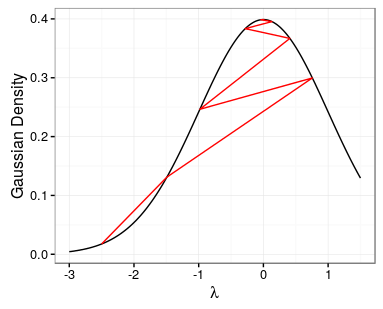
\includegraphics[width = 0.4\textwidth]{gradientascent}
\end{figure}
\end{frame}

\begin{frame}
\frametitle{Stochastic Optimisation}
\begin{itemize}
\item ELBO gradients can be estimated by the Score Estimator:
\begin{align*}
\widehat{\frac{\delta\mathcal{L}(q, \lambda)}{\delta \lambda}}_{SC} &= \sum_{j = 1}^M \frac{\delta \log(q_{\lambda}(\theta_{N+1}^{(j)} | \textbf{z}_{1:N+1}))}{\delta \lambda}  \\
&\times \left(\log(p(\theta_{N+1}^{(j)}, \textbf{z}_{1:N+1})) - \log(q_{\lambda}(\theta_{N+1}^{(j)} | \textbf{z}_{1:N+1})) \right),
\end{align*}
where $\theta_{N+1}^{(j)} \sim q_{\lambda}(\theta_{N+1} | \textbf{z}_{1:N+1})$.
\end{itemize}
\end{frame}

\begin{frame}
\frametitle{Stochastic Optimisation}
\begin{itemize}
\item Or the Reparameterised Estimator, where $\theta_{N+1} = f(\epsilon, \lambda)$:
\begin{align*}
\widehat{\frac{\delta\mathcal{L}(q, \lambda)}{\delta \lambda}}_{RP} &= \sum_{j = 1}^M \frac{\delta J(\lambda, \epsilon^{(j)})}{\delta \lambda} + \frac{\delta \theta_{N+1}}{\delta \lambda} \\
\times \frac{\delta \log(p(\theta_{N+1}, \textbf{z}_{1:N+1}))}{\delta \theta_{N+1}} \bigg\rvert_{\theta_{N+1} = f(\lambda, \epsilon^{(j)})},
\end{align*}
where $\epsilon^{(j)} \sim q(\epsilon)$.
\end{itemize}
\end{frame}

\begin{frame}
\section{Online Heterogeneous Forecasting: Problem}
\subsection{Self-Driving Vehicles}
\frametitle{Self-Driving Vehicles}
\begin{itemize}
\item Self-Driving Vehicles are a thing soon
\item The navigation system has three steps
\begin{enumerate}
\item Detect surrounding traffic
\item Forecast surrounding traffic
\item Navigate through safely
\end{enumerate}
\item Forecasting has not had much work
\end{itemize}
\end{frame}

\begin{frame}
\frametitle{Forecasting Methods}
The literature forecasts vehicles in three ways:
\begin{enumerate}
\item Constant Behaviour.
\item Predict Events.
\item Provide Point Estimates.
\end{enumerate}
\end{frame}

\begin{frame}
\frametitle{Aims of the first paper}
\begin{itemize}
\item What we plan on doing with this first paper
\item Overall goals and stuff
\item Motivate heterogeneity
\item Note heterogeneity needs inference on vehicles as they are encountered
\item There is not much time to do that
\item Develop an approximation to the Bayesian Update Equation so we can infer parameters for new vehicles online
\item Also mention something on density forecasting would be nice
\end{itemize}
\end{frame}

\begin{frame}
\subsection{The Next Generation Simulation Dataset}
\frametitle{Next Generation Simulation}
\begin{itemize}
\item This is a dataset created for macro traffic modelling
\item It records all of the cars all of the time
\item The road is curved
\item Before and After of road straightening project
\end{itemize}
\end{frame}

\begin{frame}
\frametitle{Trigonometric Motion Equations}
\begin{align}
x^*_{i, t} &= x^*_{i, t-1} + v_{i, t} \cos(\delta_{i, t}) \label{xEq}, \\
y^*_{i, t} &= y^*_{i, t-1} + v_{i, t} \sin(\delta_{i, t}) \label{yEq}.
\end{align}
Picture
\end{frame}

\begin{frame}
\frametitle{Extracting Driver Inputs}
\begin{align}
\delta_{i, t} &= 
     \begin{cases}
       \tan^{-1}\left(\frac{(y^*_{i, t} - y^*_{i, t-1})}{(x^*_{i, t} - x^*_{i, t-1})} \right)  &\quad\text{if }x^*_{i, t} \neq x^*_{i, t-1} \\
       \frac{\pi}{2} &\quad\text{if } y^*_{i, t} > y^*_{i, t-1} \mbox{ and } x^*_{i, t} = x^*_{i, t-1} \\
       -\frac{\pi}{2} &\quad\text{if } y^*_{i, t} < y^*_{i, t-1} \mbox{ and } x^*_{i, t} = x^*_{i, t-1} \\
       \delta_{i, t-1} &\quad\text{otherwise,} \\ 
     \end{cases} \label{dEq} \\
v_{i, t} &= \sqrt{(x^*_{i, t} - x^*_{i, t-1})^2 + (y^*_{i, t} - y^*_{i, t-1})^2} \label{vEq}.
\end{align}
\begin{equation}
\label{aEq}
a_{i, t} = v_{i, t} - v_{i, t-1}. 
\end{equation}
\begin{itemize}
\item Why other variables are useful
\item Acceleration is good because relative velocity / non-stationarity
\end{itemize}
\end{frame}

\begin{frame}
\frametitle{Forecasting in the framework}
\begin{itemize}
\item That is a terrible title.
\item Data is split into a training set and a test set:
\item Training vehicles are observed before driving,
\item Test vehicles are encountered while driving.
\end{itemize}
\begin{figure}
\centering
\includegraphics[width = \textwidth]{problem}
\end{figure}
\end{frame}

\begin{frame}
\subsection{Auto-regressive Models for Trajectory Forecasting}
\frametitle{Auto-regressive Models for Trajectory Forecasting}
\begin{figure}
\centering
\includegraphics[width = \textwidth]{pacf}
\end{figure}
\begin{itemize}
\item Dynamics are implemented in with bivariate AR models
\item There are three approaches:
\begin{enumerate}
\item The Homogeneous Model
\item The Independent Heterogeneous Model
\item The Clustered Heterogeneous Model
\end{enumerate}
\end{itemize}
\end{frame}

\begin{frame}
\frametitle{A Homogeneous Approach}
Talk about what is going on here
\begin{align}
a_{i, t} &= \sum_{j = 1}^p \phi_{j} a_{i, t-j} + \sigma_{\epsilon} \epsilon_{i, t} \label{aAR} \\
\delta_{i, t} &= \pi/2 + \sum_{j = 1}^q \gamma_{j} (\delta_{i, t-j} - \pi/2) + \sigma_{\eta} \eta_{i, t} \label{dAR}
\end{align}
\begin{equation*}
\label{thetaVec}
\theta = \{\phi_{1}, \dots, \phi_{p}, \gamma_{1}, \dots, \gamma_{q}, \log(\sigma^{2}_{\epsilon}), \log(\sigma^{2}_{\eta})\}.
\end{equation*}
\begin{equation}
\label{indPrior}
\theta \sim \mathcal{N}\left(\mu, \Sigma \right)
\end{equation}
\begin{itemize}
\item The Posterior
\item Why are we doing this
\end{itemize}
\end{frame}

\begin{frame}
\frametitle{The Independent Heterogeneity Model}
Maybe different drivers behave differently?
\begin{align}
a_{i, t} &= \sum_{j = 1}^p \phi_{i, j} a_{i, t-j} + \sigma_{\epsilon, i} \epsilon_{i, t} \label{aAR2} \\
\delta_{i, t} &= \pi/2 + \sum_{j = 1}^q \gamma_{i, j} (\delta_{i, t-j} - \pi/2) + \sigma_{\eta, i} \eta_{i, t}. \label{dAR2}
\end{align}
This breaks down into a bunch of independent posteriors
\begin{equation}
p(\theta_{1:N} \mid z_{1:N}) = \prod_{i=1}^N p(\theta_{i} \mid z_{i}),
\end{equation}
The training set isn't terribly useful.
\begin{equation}
p(\theta_{i}| \textbf{z}_{1:N}, z_{i,1:T}, \theta_{1:N}) = p(\theta_{i} | z_{i, 1:T}) \propto p(z_{i, 1:T} | \theta_i) p(\theta_i).
\label{indepNewCar}
\end{equation}
\end{frame}

\begin{frame}
\frametitle{The Clustered Heterogeneity Model}
Hierarchical Models share information 
\begin{itemize}
\item Introduce Auxiliary Variable K
\item Sharing of the information
\end{itemize}
\begin{equation}
\label{mixPrior}
\theta_i | k_i = j \sim N(\mu_j, \Sigma_j),
\end{equation}
and
\begin{equation}
k_i \mid \beta \sim \mbox{Multinomial}\left(\pi_1, \dots, \pi_{K}\right)
\end{equation}
\begin{align}
\mu_j &\sim \mathcal{N}\left(\bar{\mu}_j, \Omega_j\right), \\
\Sigma_j &\sim \mbox{Inverse Wishart}\left(\mbox{Degrees of Freedom } \tau_j, \mbox{Scale } \Psi_j\right), \\
\boldsymbol{\pi} &\sim \mbox{Dirichlet}\left(\alpha_1 = \alpha_2 = \dots = \alpha_K\right).
\end{align}
\end{frame}

\begin{frame}
\frametitle{The Clustered Heterogeneity Model}
The new vehicle depends on the old vehicles through $\beta$.
\begin{equation}
\label{hierNewCar}
p(\theta_{i} | \textbf{z}_{1:N}, z_{i, 1:T}) \propto p(z_{i, 1:T} | \theta_{i}) \int_{\beta} p(\theta_{i} | \beta) p (\beta | \textbf{z}_{1:N}) d\beta.
\end{equation}
The $\beta$ posterior is precise for large $N$
\begin{equation}
\label{hierNewCar2}
p(\theta_{i} | \textbf{z}_{1:N}, z_{i, 1:T}) \propto p(z_{i, 1:T} | \theta_{i}) p(\theta_{i} | \hat{\beta}).
\end{equation}
\end{frame}

\begin{frame}
\frametitle{Heterogeneity in the Model Posteriors}
\begin{figure}
\centering
\includegraphics[width = \textwidth]{HierSingleKDE}
\end{figure}
\end{frame}

\begin{frame}
\section{Updating Variational Bayes}
\frametitle{Updating Variational Bayes}
\begin{itemize}
\item Inference for self-driving vehicles needs to be fast.
\item Inference cannot slow down as the amount of data increases.
\begin{figure}[ht]
\centering
\includegraphics[width = \textwidth]{timeUpdate}
\end{figure}
\item How do we go from $q_{\lambda_S}(\theta_{i} | z_{i, 1:S})$ to $q_{\lambda_T}(\theta_{i} | z_{i, 1:T})$ for $S < T$?.
\end{itemize}
\end{frame}

\begin{frame}
\frametitle{Approximating Bayesian Updating}
\begin{itemize}
\item The Bayesian Update Equation: 
\begin{equation}
\label{updatePost}
p(\theta_{i} | z_{i, 1:T}) \propto p(z_{i, S+1:T} | \theta_{i})p(\theta_{i} | z_{i, 1:S}).
\end{equation}
\item Computation requires evaluating the joint distribution,
\begin{equation}
\label{updateJoint}
p(\theta_{i}, z_{i, 1:T}) = p(z_{i, S+1:T} | \theta_{i})p(\theta_{i} | z_{i, 1:S}).
\end{equation}
\item We will approximate the Bayesian Update Equation in VB,
\begin{equation}
\label{ApproxJoint}
\hat{p}(\theta_{i},  z_{i, 1:T}) = p(z_{i, S+1:T} | \theta_{i})q_{\lambda_S}(\theta_{i} | z_{i, 1:S}).
\end{equation}
\item Source of additional error: How close $q$ is to $p$.
\end{itemize}
\end{frame}

\begin{frame}
\frametitle{Updating Gradient Estimators}
\begin{itemize}
\item The updating score estimator:
\begin{align*}
\widehat{\frac{\delta\mathcal{L}(q, \lambda_T)}{\delta \lambda_T}}_{USC} &= \sum_{j = 1}^M \frac{\delta \log(q_{\lambda_T}(\theta_{N+1}^{(j)} | z_{N+1, 1:T}))}{\delta \lambda_T}  \\
&\times \left(\log(q_{\lambda_S}(\theta_{N+1}^{(j)} | z_{N+1, 1:S}) - \log(q_{\lambda_T}(\theta_{N+1}^{(j)} | z_{N+1, 1:T})) \right)
\end{align*}
where $\theta_{N+1}^{(j)} \sim q(\theta_{N+1} | z_{N+1, 1:T})$. 
\end{itemize}
\end{frame}

\begin{frame}
\frametitle{Updating Gradient Estimators}
\begin{itemize}
\item The updating reparameterised estimator:
\begin{align*}
\widehat{\frac{\delta\mathcal{L}(q, \lambda_T)}{\delta \lambda_T}}_{URP} &= \sum_{j = 1}^M \frac{\delta J(\lambda_T, \epsilon^{(j)})}{\delta \lambda_T} + \frac{\delta f(\lambda_T, \epsilon^{(j)})}{\delta \lambda_T} \\
&\times \frac{\delta \log(q_{\lambda_S}(\theta_{N+1} |z_{N+1, 1:S}))}{\delta \theta_{N+1}} \bigg\rvert_{\theta_{N+1} = f(\lambda_T, \epsilon^{(j)}} 
\end{align*}
where $\epsilon^{(j)} \sim q(\epsilon)$.
\end{itemize}
\end{frame}

\begin{frame}
\section{Online Heterogeneous Forecasting: Results}
\frametitle{Point Forecasts}
\begin{itemize}
\item Introduce Naive / RNN models?
\item Some stuff about point forecasts: Both pictures?
\item Note that, on average, the homogenous model is as good as others
\item Some stuff about different inference frameworks
\item MAPs are not the whole story
\end{itemize}
\end{frame}

\begin{frame}
\frametitle{Heterogeneous Variance Distributions}
\begin{itemize}
\item Some stuff about variance
\item A note on erratic driver detection
\item Two different pictures to go in here
\end{itemize}
\end{frame}

\begin{frame}
\frametitle{Updating Variational Bayes Results}
\begin{itemize}
\item Compare to regular VB
\item Time Complexity
\item Difference in logscores
\end{itemize}
\end{frame}

\begin{frame}
\section{Extensions}
\frametitle{Extending the Framework}
\begin{itemize}
\item Copula Project
\item Other Applications
\end{itemize}
\end{frame}

\end{document}